\begin{figure*}
  \centering
    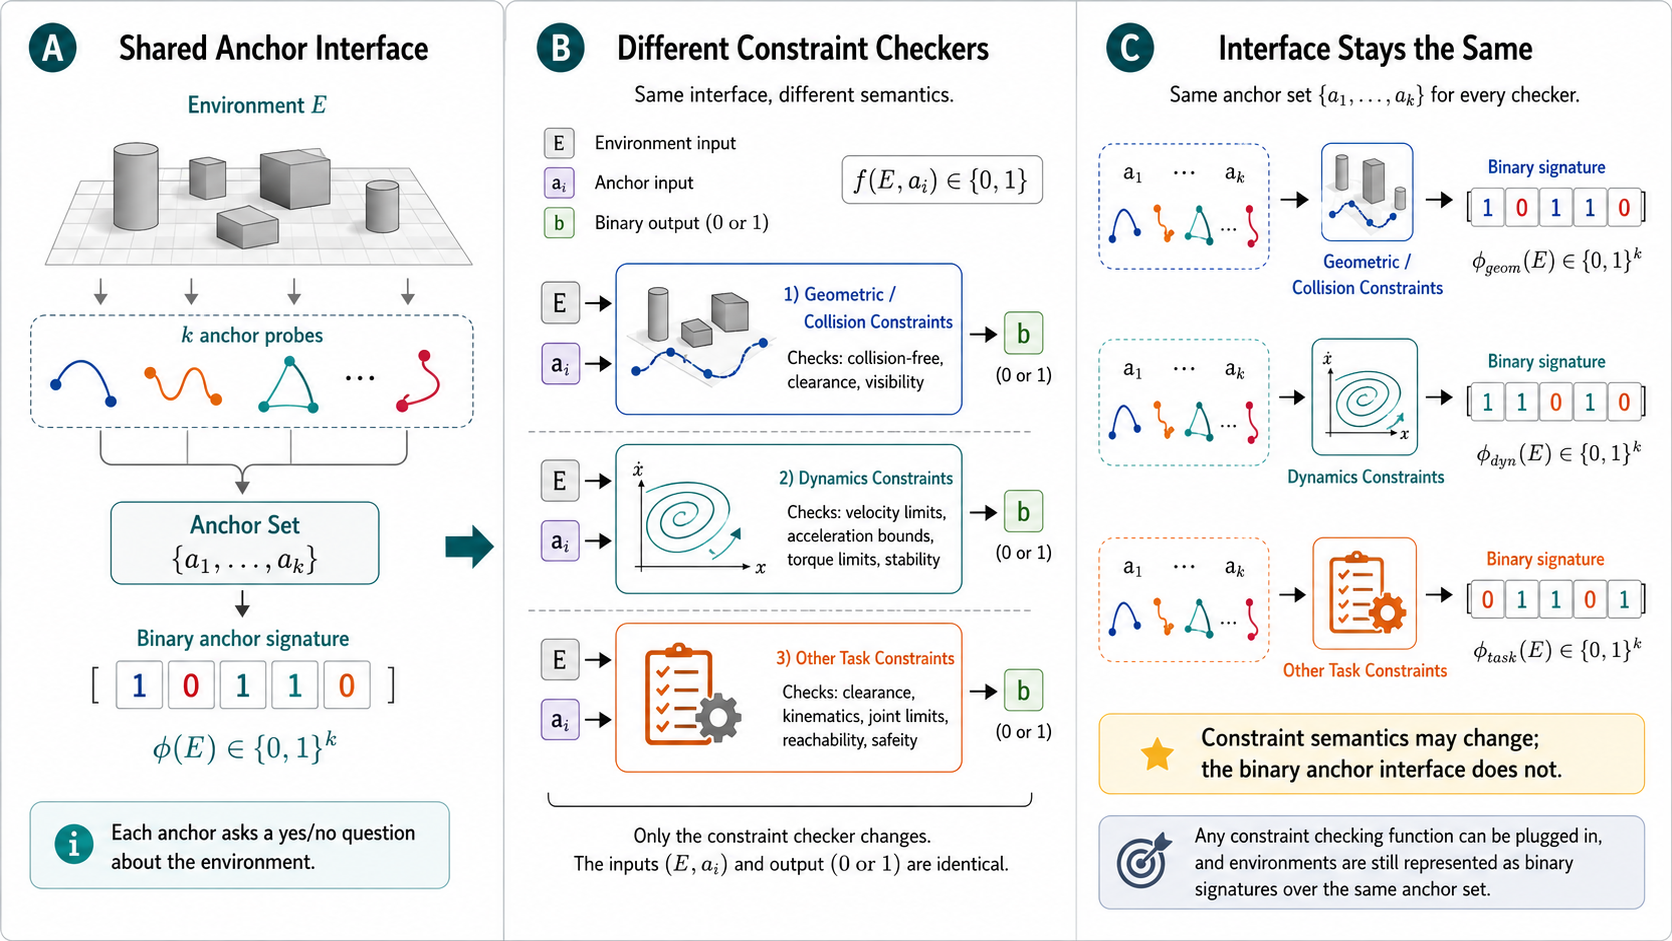
\includegraphics[width=\textwidth]{figs/explanatory.png}
  \caption{A graphical presentation of your approach. Place first thing in the second column of the first page. Refer to this image in your text.}\label{fig:first-page}
\end{figure*}

\section{Related Work}\label{sec:related-work}

\textbf{Diffusion models for robot trajectories.}
Diffusion models have recently become a powerful class of generative priors for robot decision making and trajectory generation. Diffuser formulates planning as iterative denoising over trajectories, showing that a diffusion model can represent flexible, multimodal behavior in sequential decision problems~\cite{janner2022diffuser}. Diffusion Policy extends this idea to visuomotor control by learning a conditional denoising process over action sequences and executing the generated actions in a receding-horizon manner~\cite{chi2025diffusionpolicy}. Subsequent work has improved the structure of the generated trajectories and the observation conditions used to guide denoising. ChainedDiffuser combines keypose prediction with local trajectory diffusion for manipulation~\cite{xian2023chaineddiffuser}, while 3D Diffuser Actor denoises end-effector pose trajectories conditioned on tokenized 3D scene features, language, and proprioception~\cite{ke2025threediffuseractor}. DP3 similarly argues that compact point-cloud observations provide a strong interface between 3D perception and diffusion-policy learning~\cite{ze2024dp3}. In motion planning, Motion Planning Diffusion learns trajectory priors that can seed optimization-based planners~\cite{carvalho2023motionplanningdiffusion}. These works demonstrate that diffusion models can represent expressive trajectory distributions, but they generally assume that the conditioning representation already exposes the environment differences that matter for feasible motion.

\textbf{Environment representations for learning-based planning.}
A central question in learning-based planning is how to encode the scene so that a policy or planner can generalize across environments. Early neural motion-planning work encoded workspaces from point clouds or learned obstacle features, showing that learned representations can accelerate collision-free planning in unseen scenes~\cite{strudel2021obstacle}. More recent diffusion-based planners and manipulation policies have moved toward structured 3D, object-centric, and affordance-based conditions. PRESTO represents the environment using sparse key configurations that approximate configuration-space obstacles for diffusion-based trajectory seeding~\cite{seo2024presto}. Lan-o3dp conditions a diffusion policy on language-selected, task-relevant object point clouds and uses denoising-time cost guidance for collision avoidance~\cite{li2024lano3dp}. SPOT represents manipulation tasks through object-centric SE(3) pose trajectories and uses these trajectories to condition a diffusion policy~\cite{hsu2025spot}. AffordDP further conditions diffusion policies on transferable affordances, represented through 3D contact points and post-contact trajectories, to improve generalization to novel object categories~\cite{wu2025afforddp}. These approaches reduce dependence on raw appearance by introducing geometric, object-level, or affordance-level structure. However, their abstractions are still primarily organized around what is perceived in the scene, rather than around which motions the scene permits or forbids.

\textbf{Behaviorally aligned abstraction.}
Our work is closest in spirit to representation-learning approaches that define abstraction by behavioral relevance rather than perceptual similarity. DeepMDP learns latent models whose representations preserve reward and transition structure~\cite{gelada2019deepmdp}, and deep bisimulation methods learn visual-control representations that discard task-irrelevant variation while preserving control-relevant dynamics~\cite{zhang2020invariant}. Language-guided state abstraction similarly seeks task-aligned state descriptions that suppress irrelevant observation dimensions for imitation learning~\cite{peng2024languageguided}. We adopt the same high-level principle, but instantiate it for environment-conditioned trajectory diffusion. Instead of asking a learned visual embedding to infer which perceptual differences affect planning, we define an environment through its binary responses to a fixed set of diagnostic trajectory snippets under the active constraint model. The resulting feasibility signature acts as a compact behavioral code: environments with similar feasible trajectory distributions can map to similar signatures even when they differ visually, while small perceptual changes remain separated whenever they change which trajectories are feasible. This positions our method between structured conditioning for diffusion policies and control-relevant abstraction, with the key distinction that the conditioning variable is built from explicit constraint responses rather than from perception alone.
